\chapter{Jim Rohn -- Rare Talk: Profits, Ratios, and the Structure of Change}

These notes follow Jim Rohn's fifth lecture in the present sequence, drawn from a curated playlist assembled by LazyingArt LLC rather than from a clean institutional course. The lecture begins as autobiography, but it very quickly declares a different ambition. We are asked to take notes because the speaker means to pass along a small set of operating laws. The chapter therefore keeps close to the order of the spoken argument: opportunity and philosophy first, then profits and part-time leverage, then the sailboat model of change, then the law of averages, then the sower's filter of losses, and only afterward the implementation layer of skill, service, and the good life.

\begin{remark}
No validated board screenshots survive for this lecture. The figures below are therefore cautious transcript-derived reconstructions, included only to clarify the lecture's quantitative and diagrammatic skeleton.
\end{remark}

\section{Opening Orientation: Opportunity, Product, and Philosophy}

Rohn opens by earning the right to generalize. He is the farm boy from Idaho who did not begin with many skills, who knew how to milk cows but did not know how to build a fortune, and whose life changed when he encountered a part-time marketing system joined to a product he could believe in. The family story about nutrition is not decorative. His mother taught nutrition; his grandparents passed it down; its benefits, in his telling, were visible across generations. The point is that conviction comes before technique. One stays with a field, studies it, and works through its difficulty only if one believes in what one is carrying.

This is why the lecture's first serious claim is about philosophy rather than method. Technique, product, and support do not move by themselves. A philosophy is needed to drive the person toward the necessary actions. The lecture also marks this transition theatrically. Rohn asks the audience for notes, then recalls people returning years later with old seminar notebooks still in use. That is not merely sentimental. It tells us what kind of lecture this is. A story is being turned into a reusable law.

We should therefore keep three layers distinct even when the spoken performance moves among them rapidly. The first layer is anecdote: the nutrition story, the age-twenty-five turning point, the years of struggle. The second is motivational rhetoric: take notes, keep them, use them. The third is mechanism: what exact principle changed behavior, and how does that principle propagate from one person's experience into another person's discipline? The lecture proceeds only because these three layers remain connected.

\section{Profits, Wages, and the Magic of Part Time}

Rohn announces the first law with unusual force. Profits are better than wages. He presents this not as an abstract proposition but as the line no one gave him in school and the line that, once heard, reorganized his economic life.

\begin{remark}
In this section \(W\) denotes wages and \(P\) denotes profits. The symbols are editorial shorthand for verbal lines spoken in the lecture.
\end{remark}

\begin{align}
\text{Profits are better than wages,} \qquad & P > W, \\
\text{Wages make you a living; profits make you a fortune.} \nonumber
\end{align}

The lecture briefly widens this into a rhetorical contrast between capitalism and communism. We should keep the emphasis where the speaker puts it. The point is not an independent political-economy exposition. It is the claim that capital belongs in the hands of people who can exercise ingenuity and bring goods and services to market. That widening then narrows immediately into the lecture's real mechanism: do not wait for a complete career reset. Start part time. Hold the job, but begin to work on profit.

The mentor, transcribed here as Mr.~Shove, gives Rohn the decisive sentence: full time on the job, part time on the fortune. That phrase matters because it changes the emotional meaning of labor. One is no longer only paying bills. One is beginning, even at the edge of the schedule, to build a fortune.

\begin{align}
P_{\mathrm{pt}} &= W_{\mathrm{ft}}, \\
P_{\mathrm{pt}} &= 2W_{\mathrm{ft}}.
\end{align}

These two equalities reconstruct the lecture's two milestones. First, part-time profits rise to match full-time wages. Second, part-time profits rise to double them. The lecture does not present these as timeless equations written on a board. It presents them as thresholds in a narrated life. The first threshold gives freedom of imagination: the part-time channel is now real. The second gives an invitation so powerful that Rohn says he was reluctant to go full time, because the story itself had become electrifying.

\begin{figure}[h]
\centering
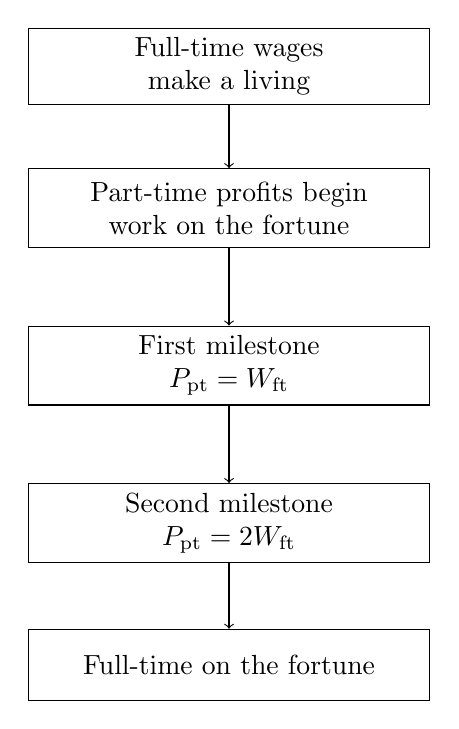
\begin{tikzpicture}
\node[draw, rectangle, align=center, minimum width=5.1cm, minimum height=0.9cm] (a) at (0,0) {Full-time wages\\make a living};
\node[draw, rectangle, align=center, minimum width=5.1cm, minimum height=1.0cm] (b) at (0,-1.8) {Part-time profits begin\\work on the fortune};
\node[draw, rectangle, align=center, minimum width=5.1cm, minimum height=1.0cm] (c) at (0,-3.8) {First milestone\\\(P_{\mathrm{pt}}=W_{\mathrm{ft}}\)};
\node[draw, rectangle, align=center, minimum width=5.1cm, minimum height=1.0cm] (d) at (0,-5.8) {Second milestone\\\(P_{\mathrm{pt}}=2W_{\mathrm{ft}}\)};
\node[draw, rectangle, align=center, minimum width=5.1cm, minimum height=0.9cm] (e) at (0,-7.6) {Full-time on the fortune};
\draw[->] (a) -- (b);
\draw[->] (b) -- (c);
\draw[->] (c) -- (d);
\draw[->] (d) -- (e);
\end{tikzpicture}
\caption{Transcript-derived reconstruction of the lecture's ``magic of part time'' ladder.}
\end{figure}

The lecture then introduces a concrete threshold for visible change:

\begin{equation}
\Delta I \approx \$1000 \text{ per month.}
\end{equation}

This is not a universal constant. It is a social marker. An extra thousand dollars a month, he says, is enough to change the lifestyle of most families quickly and visibly. That visibility is what matters.

\subsection{Question \& Answer}

Why does part-time profit become more powerful, rhetorically and practically, than ordinary full-time income?

Because the relevant variable is not cash in the abstract. It is the change in lived form. The lecture keeps returning to vacations, cars, clothes, and a new pattern of daily life. A thousand dollars a month earned full time may be absorbed into the ordinary texture of survival. A thousand dollars a month earned part time creates contrast. It tells a before-and-after story. That is why the invitation becomes credible.

\begin{equation}
\text{part-time profit} \longrightarrow \text{visible lifestyle change} \longrightarrow \text{credible invitation.}
\end{equation}

This is also why the lecture lingers on the staged milestones instead of stating only the slogan \(P>W\). Rohn wants the audience to feel how the law changes speech, invitation, and imagination.

\section{Wind, Sail, and the Possibility of Change}

From the arithmetic of profit Rohn turns to a more general model of causation. He says that what determines the future is not what happens, but what we do about what happens. The sailboat metaphor is the lecture's way of making that claim operational.

\begin{equation}
\text{It is not what happens that determines your future; it is what you do about what happens.}
\end{equation}

\begin{equation}
\text{The same wind blows on us all.}
\end{equation}

\begin{equation}
\text{The difference in arrival is not the blowing of the wind but the set of the sail.}
\end{equation}

To avoid conflict with the earlier use of \(W\) for wages, let us denote the common wind by \(\mathcal{W}\). Then the note-writer's compact summary is

\begin{equation}
A = A(S;\mathcal{W}),
\end{equation}

where \(S\) is the sail-setting and \(A\) is arrival. The lecture is not offering a physical mechanics model. It is offering a discipline of attention. If the wind is common, then explanation cannot stop at the wind. It must move to what is adjustable.

This is why Rohn immediately broadens the metaphor into history and season. The next ten years, he says, will be about like the last ten. After fall comes winter; after day comes night; after recession comes expansion; after expansion comes recession. His summary line is brief enough to function like a compact axiom:

\begin{equation}
\text{Opportunity mixed with difficulty.}
\end{equation}

Once we understand that the mix itself is stable, the lecture's next line lands with more force:

\begin{equation}
\text{For things to change, you have to change.}
\end{equation}

The transcript is noisy for one phrase in this passage, but the neighboring repetitions stabilize the intended teaching. Do not wish for fewer problems; wish for more skill. Do not wish for less challenge; wish for more wisdom. The external world is not being promised away. The lecture's claim is that agency becomes serious only when we stop waiting for history, government, bosses, or weather to do our work for us.

\begin{figure}[h]
\centering
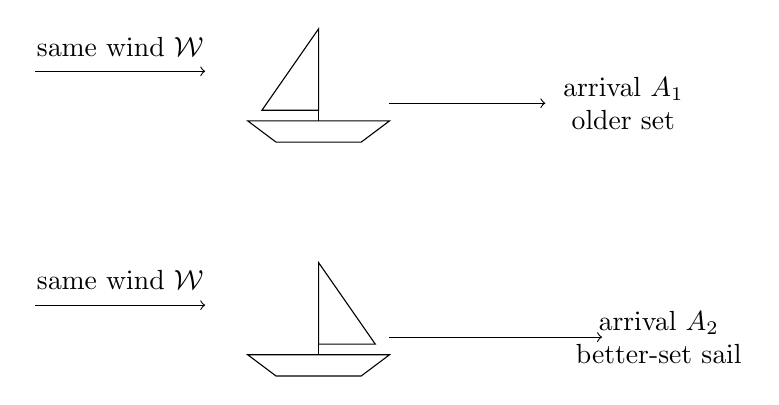
\begin{tikzpicture}[scale=0.9]
\draw[->] (-4.2,1.9) -- (-1.8,1.9);
\node at (-3.0,2.25) {same wind \(\mathcal{W}\)};

\draw (-1.2,1.2) -- (0.8,1.2) -- (0.4,0.9) -- (-0.8,0.9) -- cycle;
\draw (-0.2,1.2) -- (-0.2,2.5);
\draw (-0.2,2.5) -- (-1.0,1.35) -- (-0.2,1.35) -- cycle;
\draw[->] (0.8,1.45) -- (3.0,1.45);
\node[align=center] at (4.1,1.45) {arrival \(A_1\)\\older set};

\draw[->] (-4.2,-1.4) -- (-1.8,-1.4);
\node at (-3.0,-1.05) {same wind \(\mathcal{W}\)};

\draw (-1.2,-2.1) -- (0.8,-2.1) -- (0.4,-2.4) -- (-0.8,-2.4) -- cycle;
\draw (-0.2,-2.1) -- (-0.2,-0.8);
\draw (-0.2,-0.8) -- (0.6,-1.95) -- (-0.2,-1.95) -- cycle;
\draw[->] (0.8,-1.85) -- (3.8,-1.85);
\node[align=center] at (4.6,-1.85) {arrival \(A_2\)\\better-set sail};
\end{tikzpicture}
\caption{Transcript-derived schematic: the same wind blows on both boats, but different sail-setting produces different arrival.}
\end{figure}

\subsection{Question \& Answer}

If the world keeps sending the same wind, how can a life change drastically?

The lecture answers with Rohn's own six-year comparison. The first six years of his economic life ended in being broke; the second six years ended in being rich. He explicitly refuses the explanation that political conditions rescued him. What changed was philosophy, that is, the disciplined set of thought and action. The lecture's point is therefore sharper than mere optimism. We are not told that the wind will improve. We are told that arrival can change under the same wind.

\section{The Law of Averages as Operational Mathematics}

Once the lecture has established agency, it introduces its first explicit ratio law. If we do something often enough, a ratio appears. Once a ratio appears, it tends to continue.

\begin{equation}
\text{If you do something often enough, a ratio will appear.}
\end{equation}

\begin{equation}
\text{Once a ratio starts, it tends to continue.}
\end{equation}

In note form we write

\begin{equation}
R = \frac{s}{n},
\end{equation}

where \(n\) is the number of conversations or attempts and \(s\) is the number of affirmative outcomes. The beginner case is the lecture's own working example:

\begin{equation}
R=\frac{1}{10}.
\end{equation}

Talk to ten people; get one. The importance of the example is not statistical sophistication. It is emotional stabilization. A weak ratio does not close the game. It begins the game, because now the novice knows the law under which planning becomes possible.

\paragraph{Worked example.}
The lecture's competition example is one of its clearest derivations. Suppose an experienced person closes at nine out of ten and a beginner closes at only one out of ten. Then over a fixed contest window we can write

\begin{align}
\frac{9}{10}\cdot 10 &= 9, \\
\frac{1}{10}\cdot 100 &= 10.
\end{align}

The beginner wins, not by superior skill, but by superior volume. The speaker's own line is exact enough to preserve in display:

\begin{equation}
\text{Make up in numbers what I lack in skill.}
\end{equation}

This is the lecture's first truly worked mathematics. Skill enters through the ratio. Ambition enters through sample size. The novice is not excused from learning; he is given a way to survive until learning improves the ratio.

\begin{figure}[h]
\centering
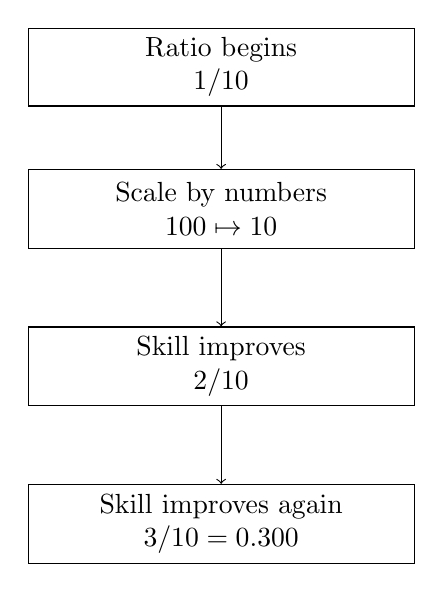
\begin{tikzpicture}
\node[draw, rectangle, align=center, minimum width=4.9cm, minimum height=0.9cm] (a) at (0,0) {Ratio begins\\\(1/10\)};
\node[draw, rectangle, align=center, minimum width=4.9cm, minimum height=1.0cm] (b) at (0,-1.8) {Scale by numbers\\\(100 \mapsto 10\)};
\node[draw, rectangle, align=center, minimum width=4.9cm, minimum height=1.0cm] (c) at (0,-3.8) {Skill improves\\\(2/10\)};
\node[draw, rectangle, align=center, minimum width=4.9cm, minimum height=1.0cm] (d) at (0,-5.8) {Skill improves again\\\(3/10 = 0.300\)};
\draw[->] (a) -- (b);
\draw[->] (b) -- (c);
\draw[->] (c) -- (d);
\end{tikzpicture}
\caption{Transcript-derived reconstruction of the lecture's law-of-averages ladder.}
\end{figure}

\subsection{Question \& Answer}

How can someone who gets only one out of ten compete with someone who gets nine out of ten?

Because the contest is not ratio alone. It is ratio together with effort. Rohn's answer is deliberately arithmetical. A worse ratio can be offset by larger \(n\). This keeps the beginner from despair, but it also avoids sentimental falsehood. The beginner is not told that he is secretly already excellent. He is told that arithmetic creates a route by which he can remain effective while skill is still low.

The law then acquires its second feature: it can improve.

\begin{equation}
\frac{1}{10} \longrightarrow \frac{2}{10} \longrightarrow \frac{3}{10}.
\end{equation}

Why does the fourth round produce two instead of one? Because, as the lecture says, we are getting better. This is why the baseball analogy is not ornamental:

\begin{equation}
0.300 = \frac{3}{10}.
\end{equation}

To bat three hundred is to fail seven times out of ten and still be elite. Hence the lecture's operational conclusion:

\begin{equation}
\text{You do not have to bat a thousand to make big money.}
\end{equation}

One out of ten is workable. Two out of ten is strong. Three out of ten is already enough, in Rohn's phrasing, to make one rich beyond prior imagination. This is also why he can tell friends to come and ``be one of the seven.'' Panic has been removed from the invitation because the averages are already understood.

\section{Sowing, Reaping, and the Structure of Loss}

A ratio law by itself could still sound too clean. We might think that once the arithmetic is known, disappointment is merely an error in execution. Rohn does not let the lecture remain there. He turns to the parable of the sower, and the parable functions here as a filter model of structured loss.

The initial conditions are favorable. The sower is ambitious. The seed is excellent. The seed may mean product, opportunity, or story. The point of the story is not that the seed was weak. The point is that even strong seed must pass through a field with losses built into it.

\begin{equation}
\text{The birds are going to get some of the seed.}
\end{equation}

The first loss channel is pre-engagement theft. Someone intended to come and did not. In the lecture's folk language, the birds got it. The wrong response is to chase birds. To chase birds is to leave the field itself.

\begin{equation}
\text{The hot weather is going to get some.}
\end{equation}

The second loss channel is early withering. Some begin, grow briefly, then disappear at the first heat. The lecture insists that we not turn this into endless inquiry. Some do not stay. One may say, with mild disappointment, ``isn't that interesting?'' but one does not rebuild the cosmos around the question.

\begin{equation}
\text{The thorns are going to get some.}
\end{equation}

The third loss channel is distraction. The thorns are the little cares, the small repairs, the screen door, the extra trash in the garage, the ordinary accumulations that choke off an opportunity before it matures. The lecture is careful here. The thorns are not dramatic villains. They are precisely the kinds of small things that cheat people out of large possibilities.

The practical line that follows is one of the chapter's strongest:

\begin{equation}
\text{You must learn to discipline your disappointment.}
\end{equation}

This line matters because it distinguishes two cases. If we made gross errors and ran people off, then correction belongs to us. But if loss occurs in the normal setup of the field, then the right response is neither rage nor metaphysical complaint. The right response is to keep sowing.

\begin{figure}[h]
\centering
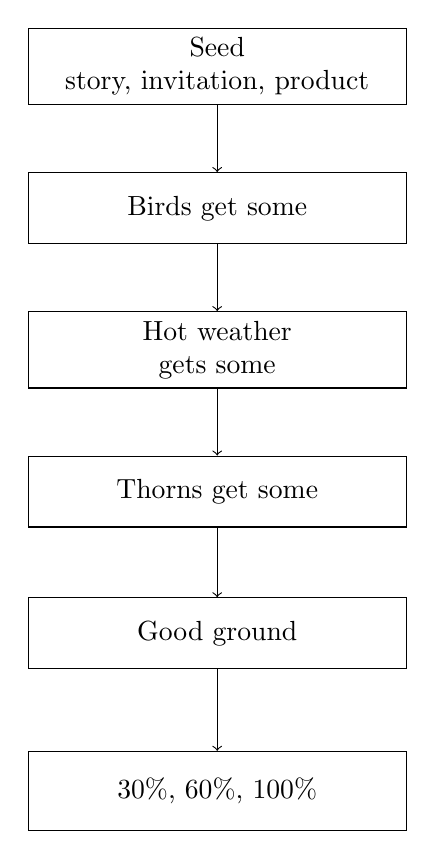
\begin{tikzpicture}
\node[draw, rectangle, align=center, minimum width=4.8cm, minimum height=0.9cm] (s) at (0,0) {Seed\\story, invitation, product};
\node[draw, rectangle, align=center, minimum width=4.8cm, minimum height=0.9cm] (b) at (0,-1.8) {Birds get some};
\node[draw, rectangle, align=center, minimum width=4.8cm, minimum height=0.9cm] (h) at (0,-3.6) {Hot weather\\gets some};
\node[draw, rectangle, align=center, minimum width=4.8cm, minimum height=0.9cm] (t) at (0,-5.4) {Thorns get some};
\node[draw, rectangle, align=center, minimum width=4.8cm, minimum height=0.9cm] (g) at (0,-7.2) {Good ground};
\node[draw, rectangle, align=center, minimum width=4.8cm, minimum height=1.0cm] (o) at (0,-9.2) {\(30\%\), \(60\%\), \(100\%\)};
\draw[->] (s) -- (b);
\draw[->] (b) -- (h);
\draw[->] (h) -- (t);
\draw[->] (t) -- (g);
\draw[->] (g) -- (o);
\end{tikzpicture}
\caption{Transcript-derived reconstruction of the sower story as a vertical filter model.}
\end{figure}

The lecture's compact structural summary is therefore

\begin{equation}
\text{Seed} \longrightarrow \text{loss channels} \longrightarrow \text{good ground} \longrightarrow \{30\%,60\%,100\%\}.
\end{equation}

The last stage is crucial. Good ground is not uniform. Some good ground does \(30\%\), some \(60\%\), some \(100\%\). Rohn's practical warning is not to force the thirties into the sixties. Let the thirties do thirty, the sixties do sixty, the hundreds do one hundred. The aim is not uniform output but durable growth.

\begin{equation}
\text{Finally, the seed falls on good ground.}
\end{equation}

\subsection{Question \& Answer}

What do we do when some do not come, some do not stay, and some are choked off by small distractions?

We do not chase birds, and we do not register for the ``why is it like this?'' class. The lecture is unusually severe on this point. One cooperates with the structure of the field. The law of averages told us that repetition yields a ratio. The sower story tells us why repetition is emotionally hard: the losses are real, recurrent, and partly outside our making. The answer is disciplined continuity. Keep sowing. If the seed is good and the sowing continues, it will eventually fall on good ground.

\section{From Philosophy to Skill: Sales, Recruiting, Organizing, Promotion, Communication}

Only after profit, wind, ratio, and sowing have been settled does the lecture turn to skill. The order matters. Otherwise the skills would read like a generic success catalog. In the spoken sequence they are the implementation layer of the earlier laws.

The first skill is sales. Rohn deliberately simplifies it. In this business sales is not a technical feat in the engineering sense. It is representation, sharing, testimony, and persuasion carried out clearly enough that the other person sees value and agrees to participate. He says that learning sales multiplied his income by five. We need not turn that into a law. It is enough to see why it appears here. Sales is the first entrepreneurial skill that converts belief into flow.

The second skill is recruiting, and here the lecture becomes more structurally ambitious. Recruiting is not merely invitation. It is invitation, presentation, and follow-up. Once a new life has started, it must be nourished and protected. This is why the lecture uses parental language. The sponsor must be mother and father at once: nourishment from one side, protection from the other.

Recruiting then receives its central image: the sponsor as bridge. The bridge carries people from darkness to light, from skepticism to faith, from discouragement to recognition. This is a decisive transition in the lecture. We are no longer describing skill merely as technique. Skill is now mediating a change of state in another person.

The third skill is organizing. Once a few people exist, the problem becomes coordination. Rohn's example is shared testimony. A new person's decision may depend less on my own story than on the story of someone standing beside me. The power lies in multiplication of credibility.

Promotion follows, and the lecture is careful to give it a local logic. The company may create major promotions, but the leader must create smaller ones. Small recognitions for small steps are what move people beyond what they would ordinarily do by themselves. This is why promotion pays, in his phrase, staggering money. The mechanism is not raw expenditure. It is ingenuity.

Communication then appears in its rawest form as an iterative discipline:

\begin{equation}
\text{I did it again.}
\end{equation}

The first talk is bad. The first movement away from the podium is awkward. The first testimony may be nearly inaudible. None of this changes the rule. One does it again. In the lecture's structure, this is the communication analogue of the ratio law and the sowing law. Repetition is not merely endurance of embarrassment. It is the process by which embarrassment is transformed into fluency.

Finally the lecture widens from communication into training, teaching, and inspiration. Training explains how the business works. Teaching explains how life works. Inspiration helps people see themselves better than they are now and more capable than they currently believe. Rohn returns here to the role his own mentor played for him: someone saw more in him than he could initially see in himself. The skills section therefore does not end in rhetoric only. It ends in a model of transmission. Philosophy becomes skill, skill becomes example, and example becomes permission for another person's change.

\section{Service, Greatness, Deserving, and the Good Life}

Recruiting already contains the seed of the lecture's next and wider question. If recruiting really changes lives, then what is the underlying law of greatness? Rohn attributes the answer first to biblical teaching, then restates it through Kennedy and Ziglar. The law is outward rather than inward.

\subsection{Question \& Answer}

How do greatness and fortune actually arise?

They arise, the lecture says, not by asking what others can do for us, but by finding a way to serve many people. In compact note form:

\begin{equation}
\text{Service to many leads to greatness.}
\end{equation}

and, schematically,

\begin{equation}
Y \uparrow \qquad \text{as} \qquad N_{\mathrm{served}} \uparrow,
\end{equation}

where \(N_{\mathrm{served}}\) is the number of people directly and indirectly affected and \(Y\) stands for pay, influence, or recognized greatness. The lecture does not give a fitted function. It gives direction. Affect a few lives and one is paid accordingly; affect many and one is paid accordingly.

Kennedy's formulation is that we should not ask what the people or country can do for us, but what we can do for them. Ziglar's formulation is the now-famous reciprocity line:

\begin{equation}
\text{If you help enough people get what they want, you can have everything you want.}
\end{equation}

Rohn then folds this broader service law back into the sponsor's daily practice. Respond to deserve, not merely to need. The lecture had already prepared this through the sower: harvest follows planting, not need alone. The sponsor's local version is an escalating response rule:

\begin{equation}
1 \mapsto 2,\qquad 2 \mapsto 5,\qquad 0 \mapsto 0.
\end{equation}

One step from the other person earns two from us; two steps earn five; no step earns no step. This is not a theorem of ethics. It is a practical allocation rule for attention and effort.

The late lecture then adds the familiar imbalance:

\begin{equation}
80\% \text{ of the people do } 20\% \text{ of the business.}
\end{equation}

The consequence is managerial rather than metaphysical. Work with a smaller portion individually and the larger portion by group. Group work is less confrontational and more scalable. That matters because there is a real limit to carrying.

\begin{equation}
\text{You can help a thousand, but you can't carry three on your back.}
\end{equation}

The companion principle is just as sharp:

\begin{equation}
\text{You cannot change people, but they can change themselves.}
\end{equation}

The pear tree remains a pear tree. Hanging apples on it does not alter what it is. This is where the lecture protects the ambitious organizer from exhausting himself in rescue fantasies. We may sponsor, teach, invite, and support. We may not substitute ourselves for the other's act of change.

Rohn then gives one more entrepreneurial sequence rule:

\begin{equation}
\text{You can either buy and sell, or sell and buy.}
\end{equation}

The point is initiative. Capital matters less than skill, courage, ingenuity, and willingness. Sometimes buying comes first. Sometimes selling creates the capacity to buy. The lecture's concern is not bookkeeping. It is that a person should not wait passively for perfect conditions before beginning.

The closing movement then shifts registers. The greatest value is not the bank account. It is the good life. The lecture's short list includes productivity, good friends, spirituality, nourishing words and culture, the inner circle, and finally participation in what he calls the miracle process. At this point the lecture becomes more ceremonial, but it does not abandon its earlier structure. It returns one last time to an economic-sounding line whose meaning is now broader than economics:

\begin{equation}
\text{If you live well, you will earn well.}
\end{equation}

This is not a claim of magic. It is a claim that a life well lived shows in voice, face, attention, magnetism, and presence. Hence the good life is not an ornament added after success. It is one of the conditions under which success becomes both sustainable and humanly intelligible.

The final dramatic note of the lecture must also be preserved. The notes themselves become a medium of presence. He goes with the audience in their notes; they go with him in his thoughts. That closing should not be flattened into generic inspiration. It is the lecture's answer to why note-taking mattered from the beginning. The laws were meant to travel.

\section{Summary}

The lecture unfolds with more internal logic than its live performance first suggests. It begins with autobiography, but only long enough to establish that opportunity without philosophy does not hold. Then it announces its first law: profits over wages, and part-time profit as the bridge from livelihood to fortune. From there it turns outward into a general model of change: common wind, variable sail. Once that is in place, the lecture becomes structurally mathematical. The law of averages supplies a ratio. The sower supplies a filter of losses. Together they explain why persistence is both rational and difficult.

Only after those laws are stable does the lecture move into skills: sales, recruiting, organizing, promotion, communication, teaching, inspiration. These are not detached tips; they are the operational layer of the earlier philosophy. The final widening then carries us from recruiting into service, from service into deserving, from deserving into the good life, and finally into the ceremonial claim that notes transmit presence. The last thing to preserve, then, is not only the equations and diagrams, but the lecture's rhythm: a law is announced, resistance is anticipated, an example is given, an obstacle is named, and then the motion resumes.